\documentclass[11pt]{article}
\usepackage[utf8]{inputenc}
\usepackage[T1]{fontenc}
\usepackage[spanish]{babel}

% Python minted
\usepackage{minted}
\usepackage{xcolor} % to access the named colour LightGray
\definecolor{LightGray}{gray}{0.95}
\setminted[python]{breaklines}

% Enumerar figuras por sección
\counterwithin{figure}{section}

% Links internos del documento
\usepackage{hyperref}

% Símbolos matemáticos
\usepackage{amsmath, amssymb, amsthm}

% Inclusión de Imágenes
\usepackage{graphicx}
\graphicspath{{Imágenes/}}
\usepackage[export]{adjustbox} % Permite añadir borde cuando se utiliza /includegraphics

% Agregación de símbolos
\usepackage{pifont}% Paquete de símbolos
\newcommand{\cmark}{\ding{51}}
\newcommand{\xmark}{\ding{55}}
\newcommand{\cbox}{\rlap{$\square$}{\raisebox{2pt}{\large\hspace{1pt}\cmark}}\hspace{-2.5pt}}
\newcommand{\xbox}{\rlap{$\square$}{\large\hspace{1pt}\xmark}}

% Viñetas enumeradas
\usepackage{enumitem}

% Double comilla \qq{}
\usepackage{textcmds} 

% No entorno flotante para imagenes \captionof{figure}{leyenda}
\usepackage{caption} 
    \captionsetup[table]{name=Tabla} % Cambiar tabla por cuadro en los caption
\usepackage{subcaption} % para subfigure

% Elimina sangría y solo usa espacio vertical respecto a los párrafos
\usepackage{parskip}

% Agregar salto de linea a \paragraph
\usepackage{titlesec}
\titleformat{\paragraph}{\normalfont\normalsize\bfseries}{\theparagraph}{1em}{\ignorespaces}
\titlespacing*{\paragraph}{0pt}{\baselineskip}{0.5\baselineskip}
%\AddToHook{cmd/section/before}{\clearpage} %Nueva página luego de una sección

% Agregar 4to nivel de indización
\setcounter{secnumdepth}{4}
\setcounter{tocdepth}{2}

% Personalización de tablas
\usepackage{booktabs}
\usepackage{colortbl} % Agregar color a la tabla
\usepackage{makecell} % Celdas con salto de línea
\usepackage{tabularx} % Tablas con ancho auto-ajustable
\usepackage{multirow}
\usepackage{array, hhline}
\newlength{\Oldarrayrulewidth}
\newcommand{\Cline}[2]{%
  \noalign{\global\setlength{\Oldarrayrulewidth}{\arrayrulewidth}}%
  \noalign{\global\setlength{\arrayrulewidth}{#1}}\cline{#2}%
  \noalign{\global\setlength{\arrayrulewidth}{\Oldarrayrulewidth}}}

% Agregar atributo H que fija definitivamente un elemento flotante.
\usepackage{float}

% Tamaño de páginas
\usepackage{geometry}
\geometry{
 a4paper,
 total={170mm,257mm},
 left=20mm,
 top=20mm,
 }

\usepackage{lipsum} 

% Agregar entorno comentario, para comentarios multilinea
\usepackage{comment}

% Colores de texto
\usepackage[dvipsnames]{xcolor}

%Generar links
\usepackage{href-ul}
\hypersetup{
    colorlinks=true,
    linkcolor=black,
    filecolor=black,
    citecolor=black,      
    urlcolor=cyan,
}
\def\UrlFont{\bfseries}

\usepackage[export]{adjustbox} % Permite añadir borde cuando se utiliza /includegraphics

% Encabezado y pie de página
\usepackage{fancyhdr}
	\pagestyle{fancy}
	\lhead{UNLP}
	\rhead{Informática}

%=======================================
% Inicio del documento
%=======================================
\begin{document}
\include{portada.tex}      % Portada de la tesis
\hypersetup{linkcolor=black}
\tableofcontents
\newpage
\hypersetup{linkcolor=black}

%=======================================
% Ejercicio 4
%=======================================
\section{Introducción}


El presente informe analítico se centra en el estudio de los patrones de deforestación y restauración forestal en la provincia de Misiones, Argentina, utilizando técnicas avanzadas de análisis matemático y estadístico. Este trabajo no solo busca comprender y cuantificar los cambios en la cobertura forestal a lo largo del tiempo, sino también aplicar modelos predictivos para anticipar tendencias futuras y evaluar el impacto de estas dinámicas en la captura de carbono y los servicios ecosistémicos.

Este informe no solo presenta un análisis detallado de los datos recopilados, sino que también demuestra la aplicación práctica de conceptos matemáticos avanzados en la resolución de problemas ambientales complejos, para ello se utilizan diversos dataset centrados en datos temporales sobre la forestacion y perdida de bosque nativo en misiones, brindadonos una oportunidad de adentrarnos en este ambito y explorar tacticas valiosas en la mitigación del cambio climático.


\subsection{Objetivos e Intereses}
La relevancia de este estudio radica en contribuir a la toma de decisiones responsables e informadas sobre forestacion, identificar areas de mejora y proporcionar datos cruciales para empresas interesadas en compensar su huella de carbono a través de créditos de CO2. Además, este análisis sirve como una herramienta de concientización sobre la explotación de los bosques nativos y sus consecuencias a largo plazo.
Desde una perspectiva matemática, este trabajo busca integrar diversos conceptos y técnicas estudiados en el curso de Matemáticas 4, entre los principales objetivos se encuentran:
\begin{enumerate}
    \item \textbf{Cuantificar y analizar los cambios en la cobertura forestal de la provincia de Misiones entre 2000 y 2022:}
    Analizar la evolución de los diferentes parámetros forestales a lo largo del tiempo utilizando visualizaciones de series temporales y estadística descriptiva.
    \item \textbf{Identificar los factores que influyen en la perdida forestal:}
    Estudiar la relación y correlación de diferentes variables como la cobertura de incendios, precipitaciones, plantaciones agropecuarias, etc.
    \item \textbf{Explorar patrones y tendencias en la deforestación y reforestación, aplicando métodos de análisis de correlación y regresión:}
    Inferir si los avances tecnológicos y las estrategias implementadas siguen una tendencia a mejorar la recuperación forestal e implementar modelos que predigan análisis futuros
    \item \textbf{Proponer acciones para mejorar la eficiencia energética y reducir el impacto ambiental:}
     Basándonos en los resultados del análisis, sugerir medidas que puedan ser implementadas por fabricantes, consumidores y gobiernos para promover el uso de practicas mas favorables con la naturaleza.
\end{enumerate}

\subsection{Consideraciones del dominio: Conceptos }
En este estudio es crucial comprender conceptos de ecologia forestal y datos geoespaciales. Para entender las dinámicas de medicion y el papel  de los ecosistemas en la mitigación del cambio climático. A continuación, se presentan los conceptos clave que guiarán este estudio:

\textbf{Conceptos básicos}
\begin{itemize}
    \item \textbf{CO2}: Dióxido de carbono
    \item \textbf{Cobertura Forestal:} Se refiere al área de tierra cubierta por árboles y otra vegetación leñosa. En nuestro conjunto de datos, esto se representa como el área total en hectáreas.
    \item \textbf{Perdida Arborea:} Es el proceso de pérdida de cobertura forestal debido a actividades humanas o por causas naturales.
    \item \textbf{Deforestación: }Es el proceso de pérdida de cobertura forestal debido a actividades humanas.
    \item \textbf{Reforestación: }Es el proceso de recuperación de la cobertura forestal, ya sea por medios naturales o por intervención humana. En nuestro conjunto de datos, esto se asocia con la columna 'gain'.
    \item \textbf{Emisiones de CO2:} Se refiere a la liberación de dióxido de carbono a la atmósfera, en este caso, como resultado de la pérdida de cobertura forestal.
    \item \textbf{Medida "ha"}: Es la abreviatura de "hectárea", una unidad de medida de superficie equivalente a 10,000 metros cuadrados. En nuestro conjunto de datos, todas las medidas de área se expresan en hectáreas.
    \item \textbf{UMD}: Metodología desarrollada por la Universidad de Maryland para estimar la pérdida de cobertura arbórea a partir de imágenes satelitales.
    \item \textbf{Cambio neto en cobertura forestal}: En nuestro conjunto de datos, la columna 'net diff' representa el obtiene un valor positivo (ganancia neta) o negativo (pérdida neta).
    \item \textbf{Tasa de recuperación:} Es la relación entre la ganancia y la pérdida forestal, indicando la capacidad del bosque para regenerarse en relación con la deforestación sufrida.
    \item \textbf{Servicios ecosistémicos: }Son los beneficios que los ecosistemas forestales proporcionan a la sociedad, incluyendo la captura de carbono, la regulación del clima, la conservación de la biodiversidad, entre otros.
\end{itemize}

\section{Datasets}
Tras una exhaustiva búsqueda de información, decidí enfocar el proyecto en una región específica de Argentina delimitada por límites naturales. Las zonas de mayor valor económico en términos de reforestación identificadas fueron:

\begin{itemize}
    \item Gran Chaco
    \item Selva Paranaense
    \item Yunga
    \item Bosque Andino Patagónico

\end{itemize}

Debido a la extensión geográfica del Gran Chaco (que abarca Salta, Chaco, Formosa y Santiago del Estero), opte por centrar el análisis en la Selva Paranaense, específicamente en la provincia de Misiones (para mayor facilidad en la obtencion de datos), que alberga la mayor parte de este ecosistema en Argentina.

\textbf{Fuentes de datos}
\begin{enumerate}
    \item \href{https://www.globalforestwatch.org}{Global Forest Watch (GFW)}: Proporciona datos globales sobre pérdida forestal y emisiones de CO2 y posee mapas están disponibles en Google Earth Engine.
    \item \href{https://www.smn.gob.ar/}{Centro Meteorológico Nacional (CMN): } Brindaron información meteorológica de las 4 estaciones en Misiones.
    \item \href{https://plataforma.argentina.mapbiomas.org/cobertura?activeBaseMap=9&layersOpacity=100&activeModule=coverage&activeModuleContent=coverage%3Acoverage_main&activeYear=2022&mapPosition=-26.504989%2C-55.085449%2C7&timelineLimitsRange=1998%2C2022&baseParams[territoryType]=2&baseParams[territories]=3%3BMisiones%3B2%3BProvincia%3B-28.16422277099997%3B-56.05864361999994%3B-25.49431473599998%3B-53.63738317999997&baseParams[activeClassTreeOptionValue]=default&baseParams[activeClassTreeNodeIds]=1%2C2%2C4%2C5%2C6%2C3&baseParams[activeSubmodule]=coverage_main}{MapBiomas}: Plataforma que ofrece datos sobre cobertura y uso del suelo a nivel regional.
    \item \href{https://www.argentina.gob.ar/ambiente/bosques/segundo-inventario-nacional-bosques-nativos}{Segundo Inventario Nacional de Bosque Nativo}: Aunque no se pudo acceder directamente a los datos, proporcionó contexto valioso.
    \item \href{https://www.argentina.gob.ar/ambiente/bosques/segundo-inventario-nacional-bosques-nativos}{Archivos shape  de la provincia de Misiones: }Utilizados para delimitar el área de estudio.
    \item \href{https://datosmacro.expansion.com/energia-y-medio-ambiente/emisiones-co2/argentina}{Datosmacro.com} ofrece diferentes datasets a nivel país como información publica, en este caso se utilizo para obtener las emisiones de CO2
\end{enumerate}

\textbf{Conjuntos de datos utilizados:
}
\begin{enumerate}
    \item     Archivo TIFF (GFW) de cobertura forestal de Argentina del 2022 (valores múltiples)
    \item Archivo TIFF (GFW) de ganancia acumulada forestal de Argentina desde el 2000 al 2020 (valores binarios 0 y 1)
    \item Archivo TIFF (GFW) de perdida acumulada forestal de Argentina desde el 2000 al 2020 (valores binarios 0 y 1)
    \item Archivo CSV  (GFW) de perdida por incendios en misiones por año
    \item Archivos TIFF (Mapbiomas) de uso de suelo anuales desde 2000 hasta 2022 de Misiones. 
    \item Archivo CSV (MapBiomas) con datos de cobertura del suelo por categorías
    \item Archivo TXT (CMN) de información meteorológica de Bernardo de Irigoyen Aero 
    \item  Archivo TXT (CMN) de información meteorológica de Iguazu Aero    
    \item Archivo TXT (CMN) de información meteorológica de Posadas Aero    
    \item Archivo TXT (CMN) de información meteorológica de  Obera
    \item Archivo CSV de emisiones de CO2 por año
    \item Archivo SHAPE de la provincia de Misiones
\end{enumerate}



\subsection{Preprocesamiento general}
En esta sección se describirá el preprocesamientos utilizados para generar el dataset, respecto a los \textbf{combinacion de parametros} y \textbf{creacion de variables}.

Para este trabajo se utilizaron las siguiente librerias en la version de python 3.12 y el motor de procesamiento de Google Earth Engine:
\begin{itemize}
    \item pandas
    \item numpy
    \item matplotlib
    \item seaborn
    \item geopandas
    \item rasterio
    \item xarray
    \item zarr
    \item scikit-learn
\end{itemize}

\newpage

\subsection{Preprocesamiento de imagenes satelitales}

Para el análisis de la deforestación en Misiones, fue necesario procesar diversos tipos de datos geoespaciales. Este preprocesamiento se realizó en dos etapas: el procesamiento local de archivos descargados .TIFF y el análisis en la plataforma Google Earth Engine.

\subsubsection{Procesamiento de archivos locales}
Se trabajó con 3 imágenes satelitales diferentes:
\begin{enumerate}
    \item Cobertura forestal de Argentina (2022)
    \item Ganancia forestal de Misiones (acumulada hasta el 2022)
    \item Pérdida forestal de Misiones (acumulada hasta el 2022)
\end{enumerate}

Para cada una de estas imágenes, se siguió el siguiente proceso:

1. \textbf{Recorte territorial}: Se utilizó la forma geométrica de la provincia de Misiones para recortar las imágenes satelitales originales, que cubrían toda Argentina. Este paso aseguró que:
   - Todos los mapas tuvieran exactamente las mismas dimensiones
   - Se redujera el tamaño de los archivos para un procesamiento más eficiente
   - Se mantuviera la coherencia espacial entre diferentes capas de datos

2. \textbf{Actualización de metadatos}: Para cada imagen recortada, se actualizaron los metadatos para reflejar:
   - Las nuevas dimensiones
   - La transformación geométrica aplicada
   - El controlador de formato de archivo (GTiff)

3. \textbf{Exportación}: Las imágenes procesadas se guardaron en formato GeoTIFF, manteniendo toda la información geoespacial necesaria para análisis posteriores.

\subsubsection{Procesamiento en Google Earth Engine} \label{sec:process_google_earth_engine}

Se trabajó con 22 imágenes satelitales de Mapbiomas (desde el año 2000 hasta el 2022 respectivamente) que separan categoricamente la cobertura de suelo.
En nuestro analisis las zonas involucradas que nos interesan son:

\begin{itemize}
    \item Cobertura Forestal: area como cojunto union de
            \begin{itemize}
                \item Vegetacion natural leñosa
                \item Vegetacion natural no leñosa
            \end{itemize}
    \item Area Agropecuaria: area como conjunto union de
    \begin{itemize}
        \item Pastura
        \item Cultivos
        \item Plantaciones
    \end{itemize}
\end{itemize}

Se implementó un algoritmo en Google Earth Engine para analizar los cambios forestales año a año:

1. \textbf{Detección de cambios}: Para cada par de años consecutivos, se:

   \begin{itemize}
       \item Identificaron las áreas que cambiaron de forestal a no forestal (pérdida)
       \item Identificaron las áreas que cambiaron de no forestal a forestal (ganancia)
   \end{itemize}

2. \textbf{Cuantificación}: Se calculó:

   \begin{itemize}
       \item  El área en hectáreas de pérdida forestal por año
       \item  El área en hectáreas de ganancia forestal por año

   \end{itemize}

Se probo que la suma de ambos debería corresponderse con el total de cobertura forestal para que no exista una discrepancia en los datos

3. \textbf{Exportación}: La colección procesada se guardaron en formato CSV, contabilizando toda la perdida y ganancia neta por año, 

\subsection{Preprocesamiento del dataset de cobertura terrestre}

La diversidad de datos nos demanda una forma de trabajar de manera consistente a través de los datasets. En este paso se realizaran las siguientes transformaciones para simplificar el análisis de variables:

\begin{itemize}
    \item Integrar las múltiples fuentes de datos en un formato analizable
    \item Crear métricas que faciliten la comprensión de la dinámica forestal
\end{itemize}

El proceso detallado fue el siguiente:

1. \textbf{Fuentes de datos combinadas}:
   \begin{itemize}
       \item  Cambios forestales calculados de ganancia y perdida \textit{\hyperref[sec:preprocesamiento]{Sección \ref{sec:process_google_earth_engine} - Preprocesamiento})}
       \item Datos de pérdida forestal por incendios
       \item Datos de cobertura de suelo de MapBiomas
   \end{itemize}

2. \textbf{Métricas agregadas}:
\begin{itemize}
    \item \textbf{Area agropecuaria} (total agriculture) : Suma de:
            \begin{itemize}
                \item Pasturas
                \item Cultivos
                \item Plantaciones
            \end{itemize}
    \item \textbf{Superficie forestal total} (total forest): Suma de:
    \begin{itemize}
        \item Vegetación natural leñosa 
        \item Vegetación natural no leñosa 
    \end{itemize}
\end{itemize}

3. \textbf{Métricas derivadas}:
   \begin{itemize}
       \item \textbf{Diferencia neta} (net diff): Balance entre pérdida y ganancia forestal
       \item \textbf{Tasa de recuperación} (recovery rate): Relación entre la ganancia y la pérdida forestal
   \end{itemize}

La combinación de estas fuentes de datos y métricas nos proporciona una base sólida para nuestro análisis posterior de la deforestación en Misiones.

\subsection{Preprocesamiento del dataset meteorológico}
Los datos meteorológicos fueron proporcionados por el Centro Meteorológico de Misiones y consisten en cuatro archivos diferentes, correspondientes a distintas estaciones meteorológicas de la provincia:

\begin{enumerate}
    \item Bernardo de Irigoyen Aero 
    \item Oberá
    \item Iguazú Aero
    \item Posadas Aero
\end{enumerate}

Cada archivo contiene registros diarios de diversos parámetros meteorológicos a lo largo de 23 años. Sin embargo, es importante notar que existe una diferencia en la cantidad de parámetros registrados entre las estaciones:

\begin{itemize}
    \item Bernardo de Irigoyen y Oberá registran 6 parámetros
    \item Iguazú y Posadas registran 9 parámetros
\end{itemize}

El resultado debe mantener la forma de los anteriores datasets, ordenados por año, para un analisis consistente se siguio el siguiente proceso

1. \textbf{Unificacion}: Para crear un dataset unificado y manejable, se leyeron los cuatro archivos y se estructuraron los datos en una matriz multidimensional para trabajar y acceder a los datos por parámetro, año y estación.

2. \textbf{Coherencia de datos}: Se estableció un mapeo común para los parámetros entre todas las estaciones, asegurando que los datos se alinearan correctamente a pesar de las diferencias en la cantidad o valores.

2. \textbf{Calculo}: Se calcularon promedios mensuales para cada estación, estos promedios mensuales se agregaron luego a nivel anual y finalmente se combinaron los datos de las cuatro estaciones, calculando un promedio para toda la provincia.

\subsection{Atributos finales}
\begin{table}[H]
\setlength{\extrarowheight}{5pt}
\setlength{\arrayrulewidth}{1.2pt}
\begin{tabularx}{\textwidth}{|>{\hsize=0.2\hsize}X|>{\hsize=0.8\hsize}X|}
\hline \rowcolor{gray!30}
\multicolumn{2}{|c|}{\textbf{Atributos Temporales}} \\
\hline
Year & Atributo entero que indica el año de la observación \\
\hline
\rowcolor{gray!30}
\multicolumn{2}{|c|}{\textbf{Atributos de Cobertura Terrestre}} \\
\hline
Total Agriculture & Atributo real que especifica el área dedicada a la agricultura en hectáreas \\
\hline
Pasture & Atributo real que especifica el área dedicada al cultivo con fin forrajeo animal en hectáreas \\
\hline
Cultivation & Atributo real que especifica el área dedicada a cultivos arbustivos en hectáreas \\
\hline
Forest plantations & Atributo real que especifica el área dedicada a especies arboreas plantadas en hectáreas \\
\hline
Total Forest & Atributo real que especifica la cobertura forestal total en hectáreas \\
\hline
Natural woody & Atributo real que especifica el área formada por arboles con cobertura superior al 65\% en hectáreas \\
\hline
Natural  non woody & Atributo real que especifica el área natural formada por cobertura herbácea o vegetal en hectáreas \\
\hline
\rowcolor{gray!30}
\multicolumn{2}{|c|}{\textbf{Atributos de Cambio Forestal}} \\
\hline
Net loss & Atributo real que especifica la pérdida forestal total en hectáreas \\
\hline
Net gain & Atributo real que especifica la ganancia forestal en hectáreas \\
\hline
Net difference & Diferencia neta en la cobertura forestal (gain - loss) en hectáreas \\
\hline
Loss from fires & Atributo real que especifica la pérdida forestal debido a incendios en hectáreas \\
\hline
Recovery rate & Tasa de recuperación forestal (gain / loss) \\
\hline
Deforestation rate & Tasa de deforestación forestal (loss / total del año anterior) \\
\hline
CO2 Emissions & Atributo real que especifica las emisiones de CO2 en megagramos (Mg) \\
\hline
\rowcolor{gray!30}
\multicolumn{2}{|c|}{\textbf{Atributos Meteorológicos}} \\
\hline
Max Temperature & Temperatura máxima promedio anual en grados Celsius (°C) \\
\hline
Min Temperature & Temperatura mínima promedio anual en grados Celsius (°C) \\
\hline
Avg Temperature & Temperatura promedio anual en grados Celsius (°C) \\
\hline
Max Humidity & Humedad relativa máxima promedio anual en porcentaje (\%) \\
\hline
Min Humidity & Humedad relativa mínima promedio anual en porcentaje (\%) \\
\hline
Avg Humidity & Humedad relativa promedio anual en porcentaje (\%) \\
\hline
Precipitations & Precipitación total anual en milímetros (mm) \\
\hline
Avg Scalar Wind & Velocidad escalar promedio del viento anual en kilómetros por hora (km/h) \\
\hline
\end{tabularx}
\end{table}

\section{Analisis exploratorio}
Con el objetivo de tener una mejor comprensión de los diferentes datos del dataset elegido, se hará un análisis detallado de los diferentes datos, observando tendencias actuales y relación entre ellos.

\subsection{Correlacion de los atributos}
Recordemos que los valores de correlación se comprenden entre -1 y 1, donde un valor cercano a 1 indica una fuerte correlación positiva, un valor cercano a -1 indica una fuerte correlación negativa y un valor cercano a 0 indica una débil o nula correlación. 
Para relacionar un atributo utilizamos el coeficiente de correlacion lineal de Pearson.
\begin{equation*}
r = \frac{S_{xy}}{\sqrt{S_{xx}S_{yy}}}
\end{equation*}
\begin{align*}
S_{xy} = \sum_{i=1}^{n} (x_i - \bar{x})(y_i - \bar{y}) && | &&
S_{xx} = \sum_{i=1}^{n} (x_i - \bar{x})^2 && | &&
S_{yy} = \sum_{i=1}^{n} (y_i - \bar{y})^2
\end{align*}

utilizando este estadístico para cada atributo contra todos los atributos, podemos conseguir la matriz de correlación (para mejorar la comprensión, inicialmente tomaremos un subconjunto para analizar)
\begin{figure}[H]
    \centering
    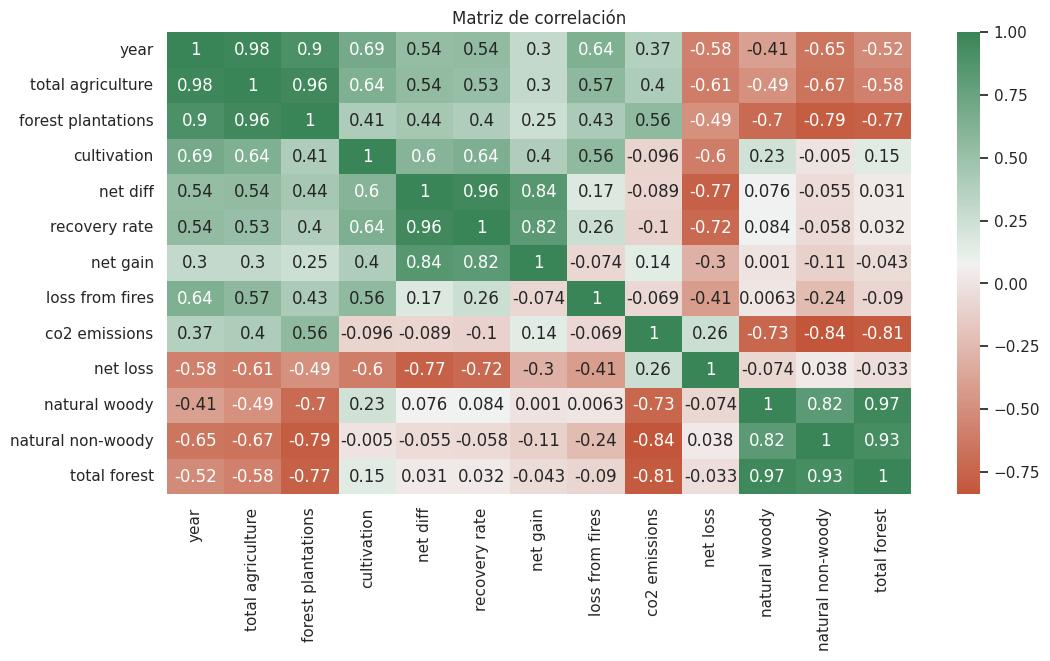
\includegraphics[width=1\linewidth, frame]{charts/correlation_matrix.jpg}
    \caption{Matriz de correlación.}
    \label{fig:matriz-correlacion}
\end{figure}

El análisis (\autoref{fig:matriz-correlacion}) revela en un primer vistazo 3 grandes grupos de variables numéricas del conjunto de datos que están fuertemente correlacionadas.

En primer lugar, se observa una correlación positiva entre ``year'', ``total agricultural'', ``Forest Plantations'' y ``cultivation''. Esto indica que el sector agricola ha aumentado significativamente con el tiempo. ``forest plantations'' encabeza su correlación con la agricultura total, esto denota que las plantaciones forestales son las que mas están creciendo y pronto veremos que ocupan gran porción del bosque nativo.

El segundo grupo se compone de ``net diff'', ``recovery rate'' y ``net gain''. Esto es lógico pues una mayor ganancia de cobertura forestal esta relacionada con la recuperación y la naturaleza de los cálculos hacen de net diff y net gain parámetros similares

El tercer grupo es entre ``natural woody'', ``natural non woody'' y``total forest''. Como las primeras 2 variables son composicion de total forest es logico que esten fuertemente relacionadas.
Tambien notamos que el area total forestal tiene correlacion negativa con los años indicando que el bosque nativo ha decrecido con el tiempo

Una de las relaciones mas llamativas se produce entre nuestras 2 variables agregadas: ``total forest'' y ``total agriculture'' (-0.58). Esto indica que a medida que aumenta el área agrícola, el área total forestal, disminuye. Este resultado puede reflejar el impacto de la expansión agrícola sobre la cobertura forestal nativa.

Una correlacion preocupante que encontramos en nuestro dataset es entre ``Loss from fires'' y ``year'' positiva, esto que significa que los incendios forestales han aumentado con el tiempo.

Como ultimo caso analizaremos la variable ``co2 emissions''. Las emisiones de CO2 están directamente relacionadas con la pérdida de cobertura forestal pues los arboles liberan el CO2 que absorben durante su vida cuando son talados y la deforestación es un factor critico en las emisiones de CO2, podemos notar que existe una correlacion negativa muy alta (-0.81) entre co2 emissions y total forest.



\subsection{Evolución temporal} \label{tab: Analisis 1 }
Para comprender las tendencias actuales de emisiones de CO2 y evolución a lo largo del tiempo, se analizarán como las deforestacion y reforestacion ha cambiado con el paso del tiempo y qué factores han sido los responsables de las tendencias actuales.

Inicialmente queremos entender la tendencia general en el total de la superficie de bosque nativo a lo largo del tiempo. Utilizando la libreria matplotlib podemos obtener un grafico para visualizar la relacion ambas etiquetas.

\begin{minted}[
baselinestretch=1.2,
bgcolor=LightGray,
fontsize=\footnotesize,
linenos]{python}
plt.figure(figsize=(12, 6))
sns.lineplot(df, x='year', y='total forest')
plt.ylabel("cobertura forestal (millones de hectareas)")
plt.show()
\end{minted}

\begin{figure}[H]
    \centering
    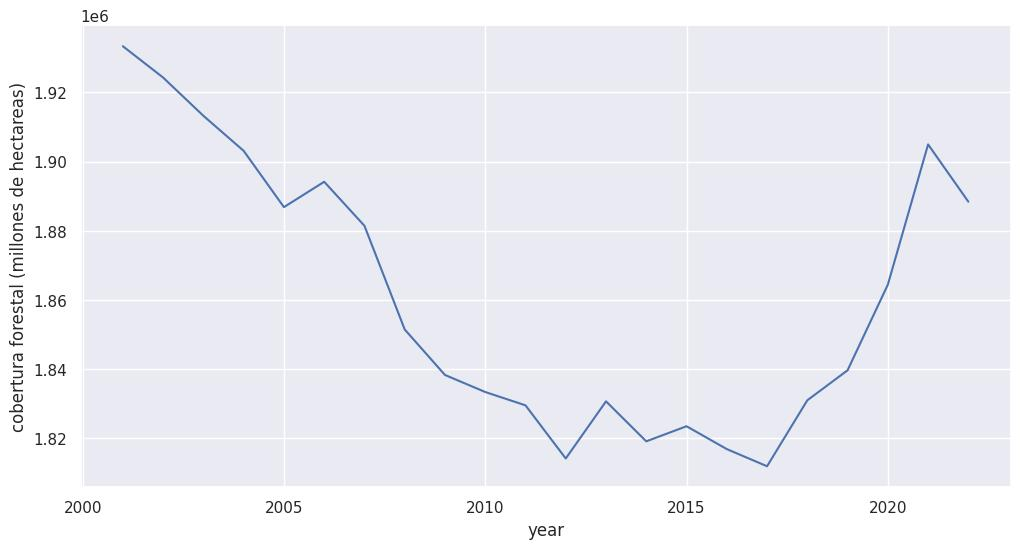
\includegraphics[width=0.78\linewidth, frame]{charts/linear--total_forest-year.jpg}
    \caption{Cobertura forestal por año.}
    \label{fig:lineal-anio-emisiones}
\end{figure}

Los datos muestran que el total de bosque nativo parece decrecer a lo largo de los años, con un 1.93 millones de hectareas en el 2000 y  1.81 millones de hectareas en su punto mas bajo 2017 (una perdida del 6.27\% de cobertura forestal). Posterior al 2017 se presenta una recuperacion hasta el 2021 (con una recuperacion del 5.13\%), esto suguiere un cambio en las politicas de forestacion o produccion, podemos considerar las restricciones en actividad economica como la tala y la expansion agricola, seguidos de menor actividad humana que se produjeron durante la pandemia de COVID-19 como un factor que pudo haber permitido a los ecosistemas forestales regenerarse. Con esto tambien podemos observar que los datos posteriores a esta etapa vuelven a dejar de ser alcistas.

\begin{figure}[H]
    \centering
    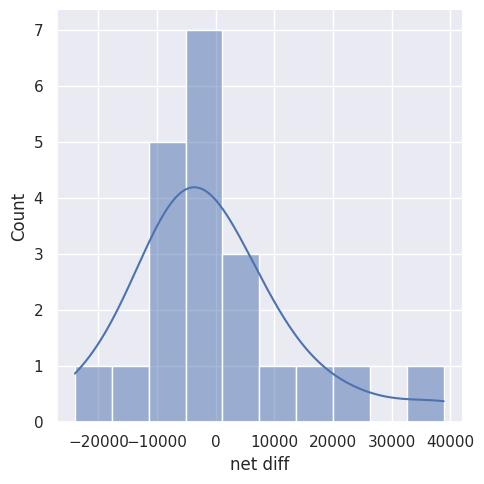
\includegraphics[width=0.5\linewidth, frame]{charts/distribution--net_diff.jpg}
    \caption{Distribucion de diferencia neta forestal por año.}
    \label{fig:tendencia-vehiculos-año}
\end{figure}

Viendo la distribucion de la diferencia neta y el grafico total se puede coincidir que la mayoría de los valores se concentran en el rango de -30,000 a 10,000. Indicando más años con pérdida de cobertura forestal que con ganancia.
\begin{figure}[H]
    \centering
    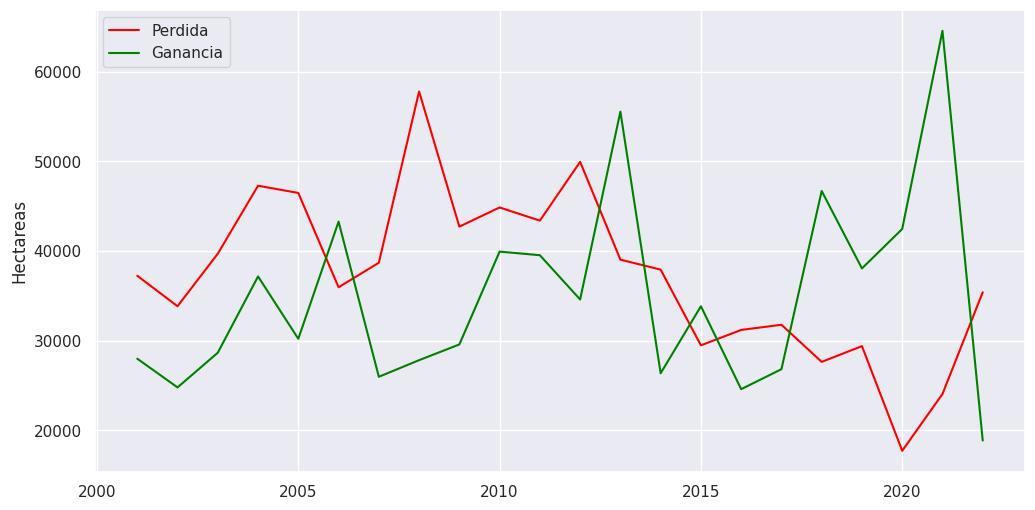
\includegraphics[width=.9\linewidth, frame]{charts/linear--gain_loss-year.jpg}
    \caption{Grafico de ganancia y perdida por año}
    \label{fig:prom-emisiones-vehiculos-año}
\end{figure}
\begin{figure}[H]
    \centering
    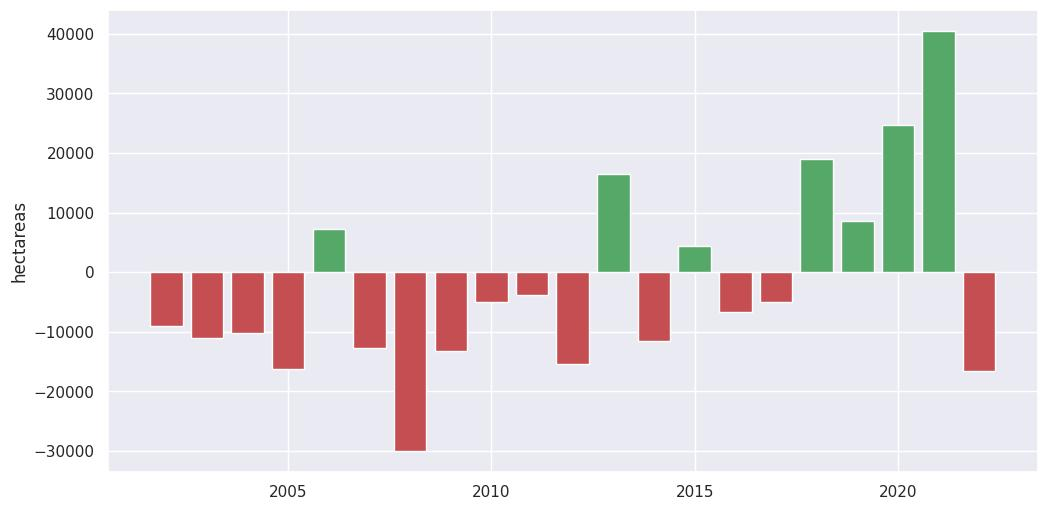
\includegraphics[width=.9\linewidth, frame]{charts/bar--recovery_rate.jpg}
    \caption{tasa derecuperacion por año}
    \label{fig:prom-emisiones-vehiculos-año}
\end{figure}

Con un grafico de perdida y ganancia forestal entendemos que la perdida no cayo muy debajo de los niveles promedio insinuando que las actividades no necesariamente hayan bajado, sin embargo las condiciones de los bosques por la menor actividad humana y un entorno mas fructuoso parecen haber impulsado su crecimiento

La relación positiva de perdida y perdida por incendio es bastante lógica. Aunque la perdida total explicada por fuego resulta ser de alrededor del 7\% por lo que nos decantamos mas por acciones humanas.

    \label{fig:prom-emisiones-vehiculos-año}
\begin{figure}[H]
    \centering
    \includegraphics[width=.9\linewidth, frame]{charts/bar--loss-loss_from_fires.jpg}
    \caption{tasa derecuperacion por año}
    \label{fig:prom-emisiones-vehiculos-año}
\end{figure}

\subsection{Análisis de Mapas Forestales} \label{tab: Analisis 2} 
Tras el análisis exploratorio temporal, procedemos a examinar la distribución espacial de la cobertura forestal, pérdida y ganancia en la provincia de Misiones. Este análisis nos permitirá visualizar patrones geográficos y entender cómo las dinámicas forestales varían a lo largo del territorio.

Para realizar este análisis, utilizamos tres conjuntos de datos geoespaciales: cobertura forestal, pérdida y ganancia. Estos datos se presentan como matrices bidimensionales, donde cada elemento representa un píxel geográfico. 
 $C$ = ``matriz de cobertura forestal'' 
 $L$ = ``matriz de pérdida''
 $G$ = ``matriz de ganancia'' 

 inicialmente vamos a mostrar los mapas y analizarlos.

\begin{figure}[H]
        \centering
        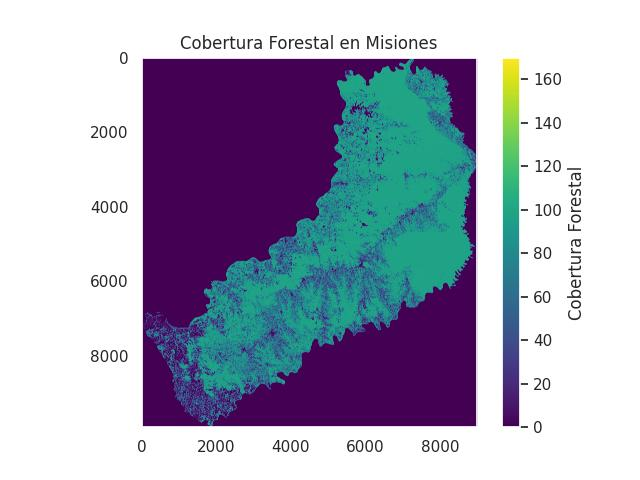
\includegraphics[width=0.9\textwidth, frame]{maps/misiones_cover.jpg}
        \caption{Mapa de cobertura forestal}
        \label{fig:smog_rating_modelos}
\end{figure}

\begin{figure}[H]
        \centering
        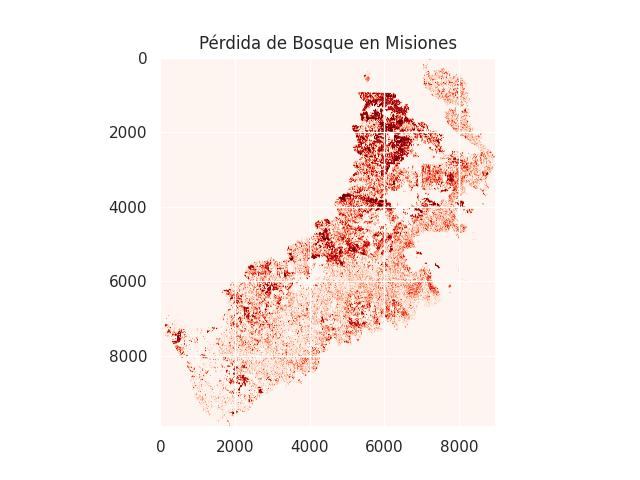
\includegraphics[width=0.9\textwidth, frame]{maps/misiones_loss.jpg}
        \caption{Mapa de perdida forestal}
        \label{fig:smog_rating_modelos}
\end{figure}

\begin{figure}[H]
        \centering
        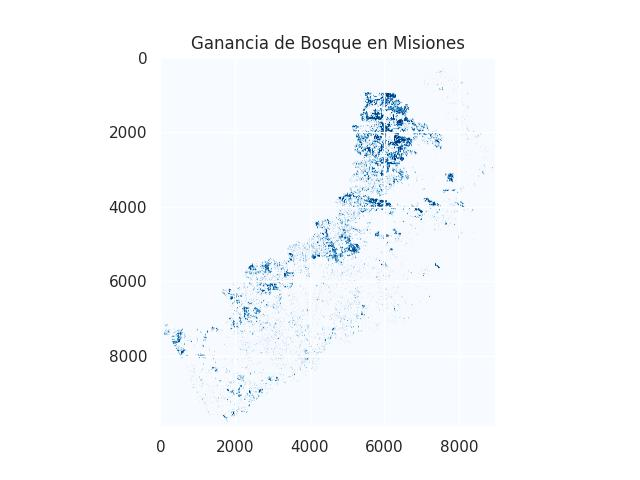
\includegraphics[width=0.9\textwidth, frame]{maps/misiones_gain.jpg}
        \caption{Mapa de ganancia forestal}
        \label{fig:smog_rating_modelos}
\end{figure}



El procesamiento de los mapas GeoTIFF implica la aplicación de operaciones matriciales y cálculos estadísticos. Inicialmente, calculamos el porcentaje de área total del mapa cubierto por bosques, utilizando la siguiente fórmula:

\begin{equation}
    \text{Cobertura Forestal} = \frac{\text{Píxeles con cobertura forestal}}{\text{Píxeles totales}} \times 100\%
\end{equation}

Cobertura Forestal = 88\%

Además del porcentaje de cobertura forestal, resulta interesante cuentificar la estructura espacial y distribución de los datos. 
Para cuantificar la estructura espacial y distribución de la cobertura forestal, inicialmente se consideró el uso del Índice de Moran y la distancia promedio entre píxeles de pérdida forestal. El Índice de Moran se define como:
\begin{equation}
    I = \frac{n}{\sum_{i}\sum_{j}w_{ij}} \cdot \frac{\sum_{i}\sum_{j}w_{ij}(x_i-\bar{x})(x_j-\bar{x})}{\sum_{i}(x_i-\bar{x})^2}
\end{equation}

Donde $n$ es el número de unidades espaciales, $w_{ij}$ son los pesos espaciales, $x_i$ es el valor de cobertura forestal en la unidad $i$, y $\bar{x}$ es la media.
La distancia promedio entre píxeles de pérdida forestal se calcula mediante:
\begin{equation}
    d = \frac{\sum_{i=1}^n d_i}{n}
\end{equation}

Donde $d_i$ es la distancia del parche $i$ a su vecino más cercano y $n$ es el número total de parches.

Sin embargo, debido a la alta resolución de nuestros datos (gran cantidad de píxeles) y la complejidad computacional asociada con estas métricas en matrices grandes, fue necesario adoptar un enfoque alternativo.

\textbf{Análisis por Clusters}
Para superar estas limitaciones y aún así obtener insights valiosos sobre la distribución espacial de la cobertura forestal, se implementó un análisis por clusters. Este método nos permite identificar y caracterizar agrupaciones significativas de cobertura forestal, pérdida o ganancia. Para cada cluster identificado, se calcularon las siguientes métricas:

Centro del cluster ($\mu$): nos indica las ubicaciones focales de la perdida forestal.
\begin{equation}\mu = (\bar{x}, \bar{y}) = (\frac{1}{n}\sum_{i=1}^n x_i, \frac{1}{n}\sum_{i=1}^n y_i)\end{equation}
Donde $(x_i, y_i)$ son las coordenadas de cada píxel en el cluster.
Desviación estándar de las distancias ($\sigma$) y varianza  ($\sigma^2$)::  Nos permiten medir la dispersión de los píxeles dentro de cada cluster, indicando si la actividad forestal está concentrada o dispersa.l
\begin{equation}\sigma = \sqrt{\frac{1}{n}\sum_{i=1}^n (d_i - \bar{d})^2}\end{equation}

Donde $d_i$ es la distancia del píxel $i$ al centro del cluster y $\bar{d}$ es la distancia media.


Densidad del cluster ($\rho$): nos da una idea de cuán compactos son los patrones de cobertura, pérdida o ganancia forestal.
\begin{equation}\rho = \frac{n}{\pi r^2}\end{equation}
Donde $n$ es el número de píxeles en el cluster y $r$ es el radio del cluster.

\begin{minted}[
baselinestretch=1.2,
bgcolor=LightGray,
fontsize=\footnotesize,
linenos]{python}
import numpy as np
from sklearn.cluster import KMeans
import matplotlib.pyplot as plt


n_clusters = 7
kmeans = KMeans(n_clusters=n_clusters, random_state=0).fit(coords_perdida)
labels = kmeans.labels_
centroids = kmeans.cluster_centers_
distances_to_centroid = np.linalg.norm(coords_perdida - centroids[labels], axis=1)

# Calcular métricas para cada cluster
for i in range(n_clusters):
    cluster_points = coords_perdida[labels == i]
    cluster_distances = distances_to_centroid[labels == i]
    
    centroid = centroids[i]
    std_dev = np.std(cluster_distances)
    variance = np.var(cluster_distances)
    density = len(cluster_points) / np.ptp(cluster_points, axis=0).prod()
    size = len(cluster_points)
    
    print(f"Cluster {i+1}:")
    print(f"Centro del cluster: {centroid}")
    print(f"Desviación estándar de las distancias: {std_dev}")
    print(f"Varianza de las distancias: {variance}")
    print(f"Densidad del cluster: {density}")
    print(f"Tamaño del cluster: {size}\n")


plt.figure(figsize=(10, 10))
plt.imshow(loss, cmap='Greens', alpha=0.5)

for i in range(n_clusters):
    cluster_points = coords_perdida[labels == i]
    plt.scatter(cluster_points[:, 1], cluster_points[:, 0], s=5, label=f'Cluster {i+1}', alpha=0.7)  # Aumentamos el tamaño y la transparencia
plt.scatter(centroids[:, 1], centroids[:, 0], c='red', s=100, marker='x', label='Centroides')  # Aumentamos el tamaño de los centroides

plt.legend(fontsize=12, loc='upper left')
plt.colorbar().remove()
plt.xlabel('Longitud')
plt.ylabel('Latitud')
plt.title('Clusters de Pérdida Forestal en Misiones', fontsize=16)
plt.grid(True, linestyle='--', alpha=0.5)

plt.show()
\end{minted}
\begin{figure}[H]
    \centering
        \centering
        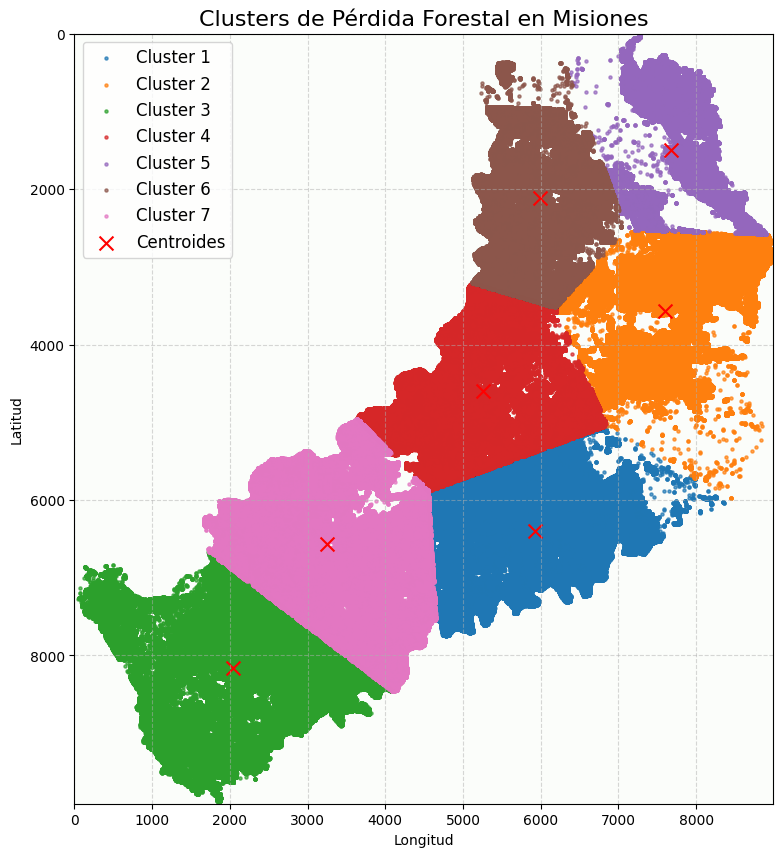
\includegraphics[width=.8\textwidth, frame]{maps/misiones_clusters_7.png}
        \caption{Mapa de perturbacion forestal - Misiones}
        \label{fig:smog_rating_año}
\end{figure}
\textbf{Cluster 1 (Azul):}
    \begin{itemize}
        \item Centro del cluster: [6401.92, 5919.88]
        \item Desviación estándar de las distancias: 367.38
        \item Varianza de las distancias: 134968.66
        \item Densidad del cluster: 0.0998
        \item Tamaño del cluster: 1028533

    \begin{table}
        \centering
        \begin{tabular}{cc}
             & \\
             & \\
             & \\
             & \\
             & \\
             & \\
        \end{tabular}
        \caption{Caption}
        \label{tab:my_label}
    \end{table}
        \end{itemize}
Este cluster se encuentra en una región con una considerable cantidad de puntos de pérdida forestal. 
La desviación estándar y la varianza indican una dispersión moderada.
La densidad sugiere que la pérdida forestal en esta área es relativamente concentrada.

\textbf{Cluster 2 (Naranja):}
    \begin{itemize}
        \item Centro del cluster: [3573.78, 7605.09]
        \item Desviación estándar de las distancias: 319.01
        \item Varianza de las distancias: 101764.82
        \item Densidad del cluster: 0.0963
        \item Tamaño del cluster: 920651
    \end{itemize}
Este cluster tiene una desviación estándar menor que el Cluster 1, lo que indica una mayor concentración de puntos cerca del centro. La densidad es ligeramente inferior, lo que puede sugerir una distribución más uniforme en el área.

\textbf{Cluster 3 (Verde):}
    \begin{itemize}
        \item Centro del cluster: [8160.25, 2041.52]
        \item Desviación estándar de las distancias: 458.43
        \item Varianza de las distancias: 210158.23
        \item Densidad del cluster: 0.0595
        \item Tamaño del cluster: 778164
    \end{itemize}
 La alta desviación estándar y varianza en este cluster indican una gran dispersión de los puntos de pérdida alrededor del centro. La densidad es la más baja entre los clusters, sugiriendo que la pérdida forestal está más distribuida y menos concentrada.
 
\textbf{Cluster 4 (Rojo):}
    \begin{itemize}
        \item Centro del cluster: [4599.58, 5256.46]
        \item Desviación estándar de las distancias: 312.44
        \item Varianza de las distancias: 97617.16
        \item Densidad del cluster: 0.1770
        \item Tamaño del cluster: 1514841
    \end{itemize}
Este cluster tiene la mayor densidad y el mayor tamaño, indicando una gran concentración de pérdida forestal en esta área. La baja desviación estándar y varianza reflejan una distribución más compacta alrededor del centro.

\textbf{Cluster 5 (Violeta):}
    \begin{itemize}
        \item Centro del cluster: [1496.12, 7671.06]
        \item Desviación estándar de las distancias: 277.46
        \item Varianza de las distancias: 76984.56
        \item Densidad del cluster: 0.0661
        \item Tamaño del cluster: 425202
    \end{itemize}
Con la menor desviación estándar y varianza, este cluster muestra la mayor concentración de puntos de pérdida cerca del centro. La baja densidad indica que, aunque los puntos están cerca entre sí, no hay tantos puntos en general comparado con otros clusters.

\textbf{Cluster 6 (Marron):}
    \begin{itemize}
        \item Centro del cluster: [2107.62, 5993.58]
        \item Desviación estándar de las distancias: 298.02
        \item Varianza de las distancias: 88813.86
        \item Densidad del cluster: 0.2777
        \item Tamaño del cluster: 1675251 puntos
    \end{itemize}
Este cluster presenta la mayor densidad, lo que indica una alta concentración de puntos de pérdida en esta área. La moderada desviación estándar y varianza sugieren una distribución relativamente compacta alrededor del centro.

\textbf{Cluster 7 (Rosa):}
    \begin{itemize}
        \item Centro del cluster: [6562.12, 3255.78]
        \item Desviación estándar de las distancias: 391.75
        \item Varianza de las distancias: 153468.51
        \item Densidad del cluster: 0.1152
        \item Tamaño del cluster: 1204592 puntos
    \end{itemize}
Este cluster muestra una dispersión considerable de los puntos de pérdida alrededor del centro, con una densidad intermedia. La alta varianza y desviación estándar indican una distribución más amplia y menos concentrada.

Este analisis revela que las áreas con mayor concentración de pérdida se encuentran en los clusters 4 y 6, y las áreas con mayor dispersión son los clusters 3 y 7 (como se intuye del mapa de perdida forestal). Esto es util para diseñar estrategias de conservación y restauración más efectivas, enfocándose en las áreas críticas del norte y entendiendo mejor la dinámica de la pérdida forestal en la región. 


Otro mapa interesante que podemos analizar es el de perturbación forestal, podemos mostrar en un mapa todos los puntos que fueron tanto ganados o perdidos.
Primero, normalizamos la matriz de cobertura forestal para que sus valores estén en el rango [0, 1]. Esto se realiza mediante la transformación lineal:

\begin{equation}
    C_{norm} = \frac{C - \min(C)}{\max(C) - \min(C)}
\end{equation}

Creación de imagen RGB:
Construimos una matriz tridimensional $R \in \mathbb{R}^{m \times n \times 3}$ para representar los canales de color Rojo, Verde y Azul. Esta construcción se puede ver como una aplicación del producto tensorial de espacios vectoriales.

$R[:,:,0] = L$ (Canal Rojo para pérdida)\\
$R[:,:,1] = 0.3  *  C_{norm}$ (Canal Verde para cobertura, reducido en intensidad)\\
$R[:,:,2] = G$ (Canal Azul para ganancia)\\

El resultado final es una función que asigna a cada par de coordenadas enteras (i, j) un vector tridimensional en el espacio de color RGB.
La visualización resultante nos permite observar simultáneamente tres aspectos clave de la dinámica forestal:

\begin{itemize}
    \item La intensidad del verde representa la densidad de la cobertura forestal.
    \item El rojo indica áreas de pérdida forestal.
    \item El azul muestra zonas de ganancia o recuperación forestal.
\end{itemize}

\begin{minted}[
baselinestretch=1.2,
bgcolor=LightGray,
fontsize=\footnotesize,
linenos]{python}
def read_raster_downsampled(filepath, factor):
    with rasterio.open(filepath) as src:
        new_width = int(src.width // factor)
        new_height = int(src.height // factor)

        data = src.read(
            out_shape=(1, new_height, new_width),
            resampling=Resampling.bilinear
        )

        data = data[0]
        return data

# Leer y reducir la resolución de los rasters
cover = read_raster_downsampled("data/misiones_cover.tif", factor=4)
gain = read_raster_downsampled("data/misiones_gain.tif", factor=4)
loss = read_raster_downsampled("data/misiones_loss.tif", factor=4)

# Normalizar la cobertura forestal
cover_norm = (cover - np.min(cover)) / (np.max(cover) - np.min(cover))

# Crear una imagen RGB
rgb = np.zeros((cover.shape[0], cover.shape[1], 3))
rgb[:,:,1] = cover_norm * 0.3  # Canal verde para cobertura forestal (reducido en intensidad)
rgb[:,:,0] = loss # Canal rojo
rgb[:,:,2] = gain # Canal azul

rgb = np.clip(rgb, 0, 1)

# Crear la figura, los ejes y mostramos la imagen
fig, ax = plt.subplots(figsize=(12, 8))
im = ax.imshow(rgb)

# Crear una leyenda personalizada
from matplotlib.patches import Patch
legend_elements = [
    Patch(facecolor='green', edgecolor='none', label='Cobertura Forestal'),
    Patch(facecolor='red', edgecolor='none', label='Pérdida de Bosque'),
    Patch(facecolor='blue', edgecolor='none', label='Ganancia de Bosque'),
    Patch(facecolor='pink', edgecolor='none', label='Perturbacion de Bosque')

]
ax.legend(handles=legend_elements, loc='lower right')

plt.title("Cobertura, Pérdida y Ganancia de Bosque en Misiones")
plt.show()
\end{minted}

\begin{figure}[H]
    \centering
        \centering
        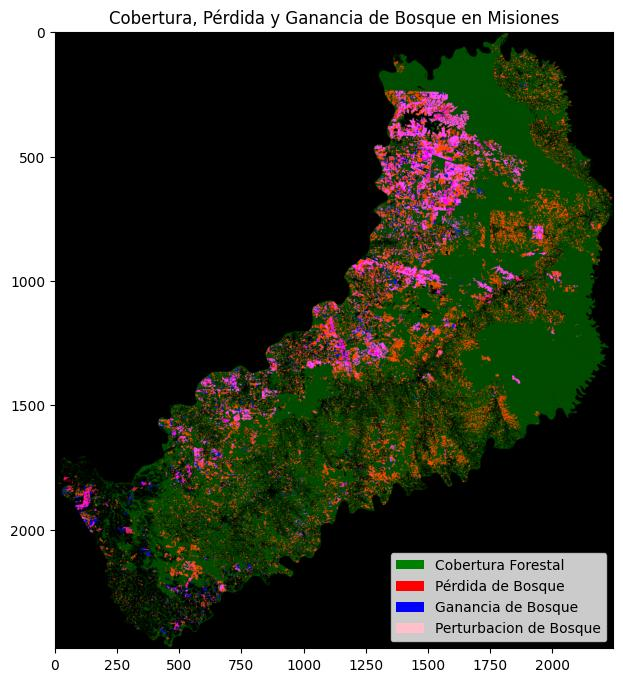
\includegraphics[width=.9\textwidth, frame]{maps/disturbed_map.jpg}
        \caption{Mapa de perturbacion forestal - Misiones}
        \label{fig:smog_rating_año}
\end{figure}

El mapa señala que la zona norta de la provincia (separada por la ruta 14) contiene la mayor perturbacion a nivel provincial, pero aunque recibe grandes perdidas tambien parece centrar su interes en la ganancia, a diferencia de la zona sur que a pesar de tener mucha menor perdida, esta es final y con poca o nula recuperacion.


\subsection{Factores influyentes en deforestacion } \label{tab: Analisis 2}
Para entender los factores que influyen en la deforestación en la provincia de Misiones, Argentina, realizaré un análisis detallado utilizando diversas variables ambientales y socioeconómicas. Los parámetros considerados son:

    \begin{itemize}
        \item Población: La densidad de población y el crecimiento demográfico pueden tener un impacto significativo en la deforestación, ya que el aumento de la población puede llevar a una mayor demanda de tierras para la agricultura, vivienda e infraestructura.
        \item Precipitaciones Totales: Las variaciones en la cantidad de lluvia pueden afectar la salud y el crecimiento de los bosques, así como influir en las prácticas agrícolas que pueden llevar a la deforestación.
        \item Humedad Relativa: Este factor climático puede influir en la susceptibilidad de los bosques a incendios y enfermedades, así como en la capacidad de regeneración de la vegetación.
        \item Radiación Solar: La cantidad de radiación solar recibida puede afectar el crecimiento de la vegetación y la productividad agrícola, lo que a su vez puede influir en la deforestación.
        \item Velocidad del Viento: El viento puede tener efectos directos e indirectos sobre los bosques, incluyendo la dispersión de incendios y la erosión del suelo.
        \item Temperatura Promedio: Las variaciones en la temperatura pueden afectar la salud de los bosques y la distribución de especies vegetales, así como influir en la agricultura.
        \item Incendios: La frecuencia y extensión de los incendios forestales son factores críticos que afectan directamente la pérdida de cobertura forestal.
        \item Agricultura: La expansión de tierras agrícolas es una de las principales causas de la deforestación. Es importante analizar la relación entre la expansión agrícola y la pérdida de bosques.
    \end{itemize}

Para llevar a cabo este análisis, se utilizarán técnicas de análisis de correlación y regresión para identificar la relación entre estos factores y la deforestación. Además, se evaluarán posibles patrones espaciales y temporales en los datos para entender mejor las dinámicas de la deforestación en la región.


\section{Modelo de predicción}

Para abordar la compleja tarea de predecir la deforestación en la provincia de Misiones, emplearemos un modelo de regresión polinómica. Este enfoque nos permite capturar relaciones no lineales entre nuestras variables predictoras y la variable objetivo, que en este caso es la pérdida de cobertura forestal.

\subsection{Explicación del modelo}

La regresión polinómica es una extensión de la regresión lineal que introduce términos de mayor orden para modelar relaciones no lineales entre variables. La ecuación general del modelo se puede expresar como:

\begin{equation}
y = \beta_0 + \beta_1x_1 + \beta_2x_2 + ... + \beta_nx_n + \beta_{11}x_1^2 + \beta_{22}x_2^2 + ... + \beta_{nn}x_n^2 + \epsilon
\end{equation}

Donde:
\begin{itemize}
\item $y$ es la variable dependiente (pérdida de cobertura forestal)
\item $x_1, x_2, ..., x_n$ son las variables independientes (población, precipitaciones, humedad, etc.)
\item $\beta_0, \beta_1, ..., \beta_n, \beta_{11}, ..., \beta_{nn}$ son los coeficientes del modelo
\item $\epsilon$ es el término de error aleatorio
\end{itemize}

Para estimar los coeficientes del modelo, utilizaremos el método de mínimos cuadrados, que busca minimizar el error entre nuestra predicción $f_{w,b}(x^{(i)})$ y el valor verdadero $y^{(i)}$. A esta medida la llamamos costo $J(w,b)$. Al entrenarlo medimos el costo de todas nuestras variables  $x^{(i)},y^{(i)}$

Para estimar los coeficientes del modelo, utilizamos el método de mínimos cuadrados ordinarios, que busca minimizar la suma de los cuadrados de las diferencias entre las predicciones del modelo $h_\beta(x^{(i)})$ y los valores observados $y^{(i)}$ . Definimos la función de costo $J(\beta)$ como:

\begin{equation}
J(\beta) = \frac{1}{2m} \sum\limits_{i = 1}^{m} (h_\beta(x^{(i)}) - y^{(i)})^2
\end{equation}

Para explicar la función de hipótesis $h_\beta(x^{(i)})$ necesitamos la matriz de características polinómicas y el vector de coeficientes

Primero, normalizamos nuestras variables predictoras para que todas estén en la misma escala. Esto es crucial para el correcto funcionamiento del algoritmo de descenso de gradiente.
\begin{equation}
X_{normalized} = \frac{X - \mu_X}{\sigma_X}
\end{equation}
Donde $\mu_X$ es la media y $\sigma_X$ es la desviación estándar de cada variable y X la matriz de caracteristicas original.

Luego creamos características polinómicas para capturar las relaciones no lineales. 
La matriz de características polinómicas se define como:
\begin{equation}
X_{poly} = [X_{normalized}, (X_{normalized})^2, \ldots, (X_{normalized})^d]
\end{equation}
Donde $d$ es el grado máximo del polinomio. Con esto podemos definir $h_\beta(x^{(i)})$ como:

\begin{equation}
h_\beta(x^{(i)}) = X_{poly}^{(i)} \cdot \beta
\end{equation}


Para minimizar la función de costo, empleamos el algoritmo de descenso de gradiente. Este método iterativo actualiza los coeficientes en la dirección opuesta al gradiente de la función de costo:

\begin{align*} 
\text{Repetir hasta convergencia:} \; \lbrace \\
\beta_j &= \beta_j - \alpha \frac{\partial J(\beta)}{\partial \beta_j} \quad \text{para } j = 0, 1, \ldots, n \\ 
\rbrace
\end{align*}

Donde:
\begin{itemize}
\item $\alpha$ es la tasa de aprendizaje
\item $\frac{\partial J(\beta)}{\partial \beta_j}$ es la derivada parcial de la función de costo con respecto a $\beta_j$
\end{itemize}

El gradiente se calcula como:

\begin{equation}
\frac{\partial J(\beta)}{\partial \beta_j} = \frac{1}{m} \sum\limits_{i = 1}^{m} (h_\beta(x^{(i)}) - y^{(i)}) \cdot x_j^{(i)}
\end{equation}



Finalmente evaluaremos el  rendimiento del modelo utilizando diferentes metricas como el error cuadrático medio, el coeficiente de determinación ($R^2$).

1. Error Cuadrático Medio (MSE):
\begin{equation}
MSE = \frac{1}{m} \sum\limits_{i = 1}^{m} (h_\beta(x^{(i)}) - y^{(i)})^2
\end{equation}

2. Coeficiente de determinación ($R^2$):
\begin{equation}
R^2 = 1 - \frac{\sum\limits_{i = 1}^{m} (y^{(i)} - h_\beta(x^{(i)}))^2}{\sum\limits_{i = 1}^{m} (y^{(i)} - \bar{y})^2}
\end{equation}
Donde $\bar{y}$ es la media de los valores observados.

\section{Modelo de predicción}

Para abordar la tarea de predecir la deforestación en la provincia de Misiones, emplearemos un modelo de regresión lineal múltiple. Este enfoque nos permite capturar las relaciones entre nuestras variables predictoras y la variable objetivo, que en este caso es la cobertura forestal total.

\subsection{Explicación del modelo}

La regresión lineal múltiple es un método estadístico que permite modelar la relación entre varias variables independientes y una variable dependiente. La ecuación general del modelo se puede expresar como:

\begin{equation}
y = \beta_0 + \beta_1x_1 + \beta_2x_2 + ... + \beta_nx_n + \epsilon
\end{equation}

Donde:
\begin{itemize}
\item $y$ es la variable dependiente (cobertura forestal total)
\item $x_1, x_2, ..., x_n$ son las variables independientes:
  \begin{itemize}
  \item Velocidad escalar promedio del viento
  \item Humedad mínima
  \item Temperatura promedio
  \item Año
  \item Superficie agrícola total
  \end{itemize}
\item $\beta_0, \beta_1, ..., \beta_n$ son los coeficientes del modelo
\item $\epsilon$ es el término de error aleatorio
\end{itemize}

\subsection{Procesamiento de datos}

Antes de aplicar el modelo, realizamos los siguientes pasos de preprocesamiento:

1. Dividimos los datos en conjuntos de entrenamiento (80\%) y prueba (20\%) para evaluar el rendimiento del modelo:

\begin{equation}
X_{train}, X_{test}, y_{train}, y_{test} = \text{train\_test\_split}(X, y, \text{test\_size}=0.2)
\end{equation}

2. Normalizamos las variables predictoras para que todas estén en la misma escala utilizando la estandarización:
\begin{equation}
X_{normalized} = \frac{X - \mu_X}{\sigma_X}
\end{equation}
Donde $\mu_X$ es la media y $\sigma_X$ es la desviación estándar de cada variable.

\subsection{Entrenamiento del modelo}

Para estimar los coeficientes del modelo, utilizamos el método de mínimos cuadrados ordinarios, que busca minimizar la suma de los cuadrados de las diferencias entre las predicciones del modelo $h_\beta(x^{(i)})$ y los valores observados $y^{(i)}$. La función de costo $J(\beta)$ se define como:

\begin{equation}
J(\beta) = \frac{1}{2m} \sum\limits_{i = 1}^{m} (h_\beta(x^{(i)}) - y^{(i)})^2
\end{equation}

Donde $h_\beta(x^{(i)})$ es la función de hipótesis:

\begin{equation}
h_\beta(x^{(i)}) = \beta_0 + \beta_1x_1^{(i)} + \beta_2x_2^{(i)} + ... + \beta_nx_n^{(i)}
\end{equation}

\subsection{Resultados del modelo}

Después del entrenamiento, obtuvimos los siguientes coeficientes:

\begin{itemize}
\item Intercepto ($\beta_0$): 1,859,905.38
\item Velocidad escalar promedio del viento ($\beta_1$): -8,378.13
\item Humedad mínima ($\beta_2$): 11,168.78
\item Temperatura promedio ($\beta_3$): 6,016.04
\item Año ($\beta_4$): -74,169.42
\item Superficie agrícola total ($\beta_5$): 38,282.98
\end{itemize}

\subsection{Evaluación del modelo}

Para evaluar el rendimiento del modelo, utilizamos dos métricas principales:

1. Error Cuadrático Medio (MSE):
\begin{equation}
MSE = \frac{1}{m} \sum\limits_{i = 1}^{m} (h_\beta(x^{(i)}) - y^{(i)})^2 = 242,856,827.00
\end{equation}

2. Coeficiente de determinación ($R^2$):
\begin{equation}
R^2 = 1 - \frac{\sum\limits_{i = 1}^{m} (y^{(i)} - h_\beta(x^{(i)}))^2}{\sum\limits_{i = 1}^{m} (y^{(i)} - \bar{y})^2} = 0.8766
\end{equation}

El valor de $R^2$ de 0.8766 indica que nuestro modelo explica aproximadamente el 87.66\% de la variabilidad en los datos, lo que sugiere un buen ajuste general.

\subsection{Interpretación del modelo}

Los coeficientes del modelo nos proporcionan información valiosa sobre la relación entre cada variable predictora y la cobertura forestal:

1. El aumento en la superficie agrícola total tiene el mayor impacto positivo en la predicción.
2. La humedad mínima y la temperatura promedio también tienen una relación positiva con la cobertura forestal.
3. El año tiene una fuerte relación negativa, lo que sugiere una tendencia general de disminución de la cobertura forestal con el tiempo.
4. La velocidad del viento tiene un impacto negativo menor en la cobertura forestal.

\section{Conclusiones}

 
\end{document}